% Geometry, font
\documentclass[12pt, letter]{article}
\usepackage[margin=0.8in]{geometry}
\usepackage[T1]{fontenc}
\usepackage{fourier}
\usepackage{titling}
\setlength{\droptitle}{-5em} 
\usepackage[parfill]{parskip}
\usepackage{graphicx}
\graphicspath{{imgs/}}
\usepackage{hyperref}

% Math stuff
\usepackage{amssymb}
\usepackage{bm}

% Code Highlighting
\usepackage{minted}
\usemintedstyle{solarizedlight}

\author{Zach Neveu}
\title{ Day 15 Notes }

\begin{document}
\maketitle

\section{Agenda}%
\label{sec:agenda}
\begin{itemize}
	\item Wrap up advanced ILP techniques
	\item Applying branch and bound
\end{itemize}

\section{Advanced LP Techniques}%
\label{sec:advanced_lp_techniques}
\begin{itemize}
	\item Review of cutting plane example from day 14.
\end{itemize}

\section{Branch and Bound Beyond ILP}%
\label{sec:branch_and_bound_beyond_ilp}
\begin{itemize}
	\item Job scheduling problem
	\item Given a set of jobs to process.
	\item Each job takes the same amount of time to process.
	\item Setup time depends on the current job and the previous job
	\item Goal: minimize total time - same as minimizing setup time
	\item Brute force - $O(n!)$
\end{itemize}

\begin{table}[h]
	\centering
	\caption{Job Scheduling Example Problem}
	\label{tab:label}
	\begin{tabular}{|c|c|c|c|c|c|}
	\hline
	Type & 1 & 2 & 3 & 4 & 5 \\
	\hline
	None & 4 & 5 & 8 & 9 & 4 \\
	\hline
	1 & 0 & 7 & 12 & 10 & 9 \\
	\hline
	2 & 6 & 0 & 10 & 14 & 11 \\
	\hline
	3 & 10 & 11 & 0 & 12 & 10 \\
	\hline
	4 & 7 & 8 & 15 & 0 & 7 \\
	\hline
	5 & 12 & 9 & 8 & 16 & 0 \\
	\hline
	\end{tabular}
\end{table}

\begin{itemize}
	\item Branch and Bound technique
	\item Possible starting bounds
	\begin{itemize}
		\item $-\infty$
		\item 0
		\item min value * num jobs - $20$ in this case
		\item $\sum$ min value in each column - $30$ in this case
		\item Can't easily tighten this now, but as tree progresses can tighten quickly
	\end{itemize}
	\item Assume schedule begins with (3,1) - cost so far $8 + 10 = 18$
	\item To compute bound, eliminate rows \texttt{none} and \texttt{3} 
	\item Take minimum from remaining problems excepting these rows
	\item Optimistic bound $8 + 10 + 7 + 10 + 7 = 42$
	\item This bound is infeasible solution - jobs 2 and 4 both done directly after job 1
	\item This seems similar to the infeasible optimistic bounds from solving ILP using LP!
	\item If bound is feasible, then this path is fathomed!
\end{itemize}

\begin{figure}[h]
	\centering
	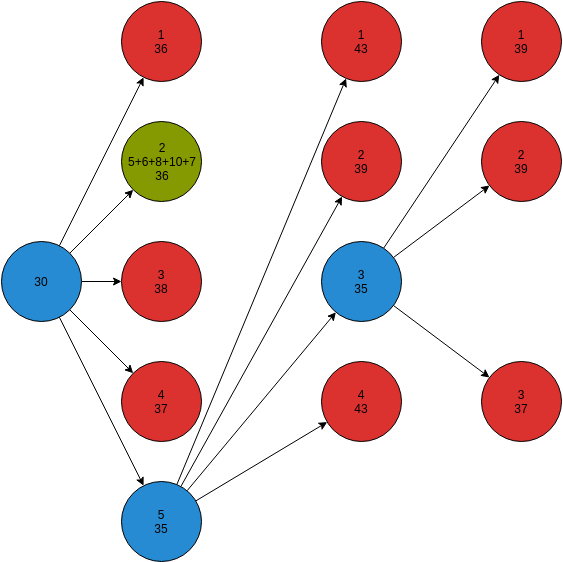
\includegraphics[width=0.8\textwidth]{jobsched}
	\caption{Job Scheduling Search Tree}
	\label{fig:jobsched}
\end{figure}

\subsection*{Knapsack w/ Branch \& Bound}
\begin{table}[h]
	\centering
	\caption{Knapsack Instance, cost limit = 100}
	\label{tab:label}
	\begin{tabular}{|c|c|c|c|c|c|c|}
	\hline
	 & 1 & 2 & 3 & 4 & 5 & 6 \\
	\hline
	$v_i$ & 10 & 35 & 40 & 18 & 2 & 4 \\
	\hline
	$w_i$ & 10 & 50 & 100 & 45 & 5 & 20 \\
	\hline
	ratio & 1 & 0.7 & 0.4 & 0.4 & 0.2 \\
	\end{tabular}
\end{table}
\begin{itemize}
	\item Sort by value/weight ratio
	\item Start tree at highest ratio item
	\item Optimistic bound: 
\end{itemize}
\begin{figure}[h]
	\centering
	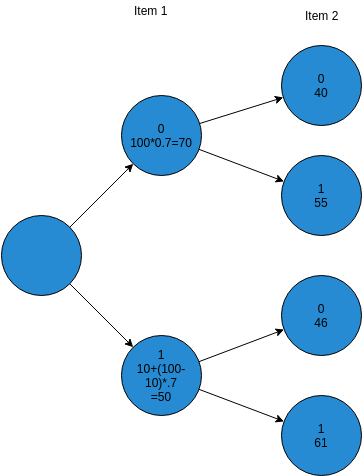
\includegraphics[width=0.8\textwidth]{knapsack}
	\caption{Knapsack Example}
	\label{fig:knapsack}
\end{figure}
\end{document}
